\documentclass{standalone}
\usepackage{tikz}
\usetikzlibrary{patterns, positioning}


\begin{document}
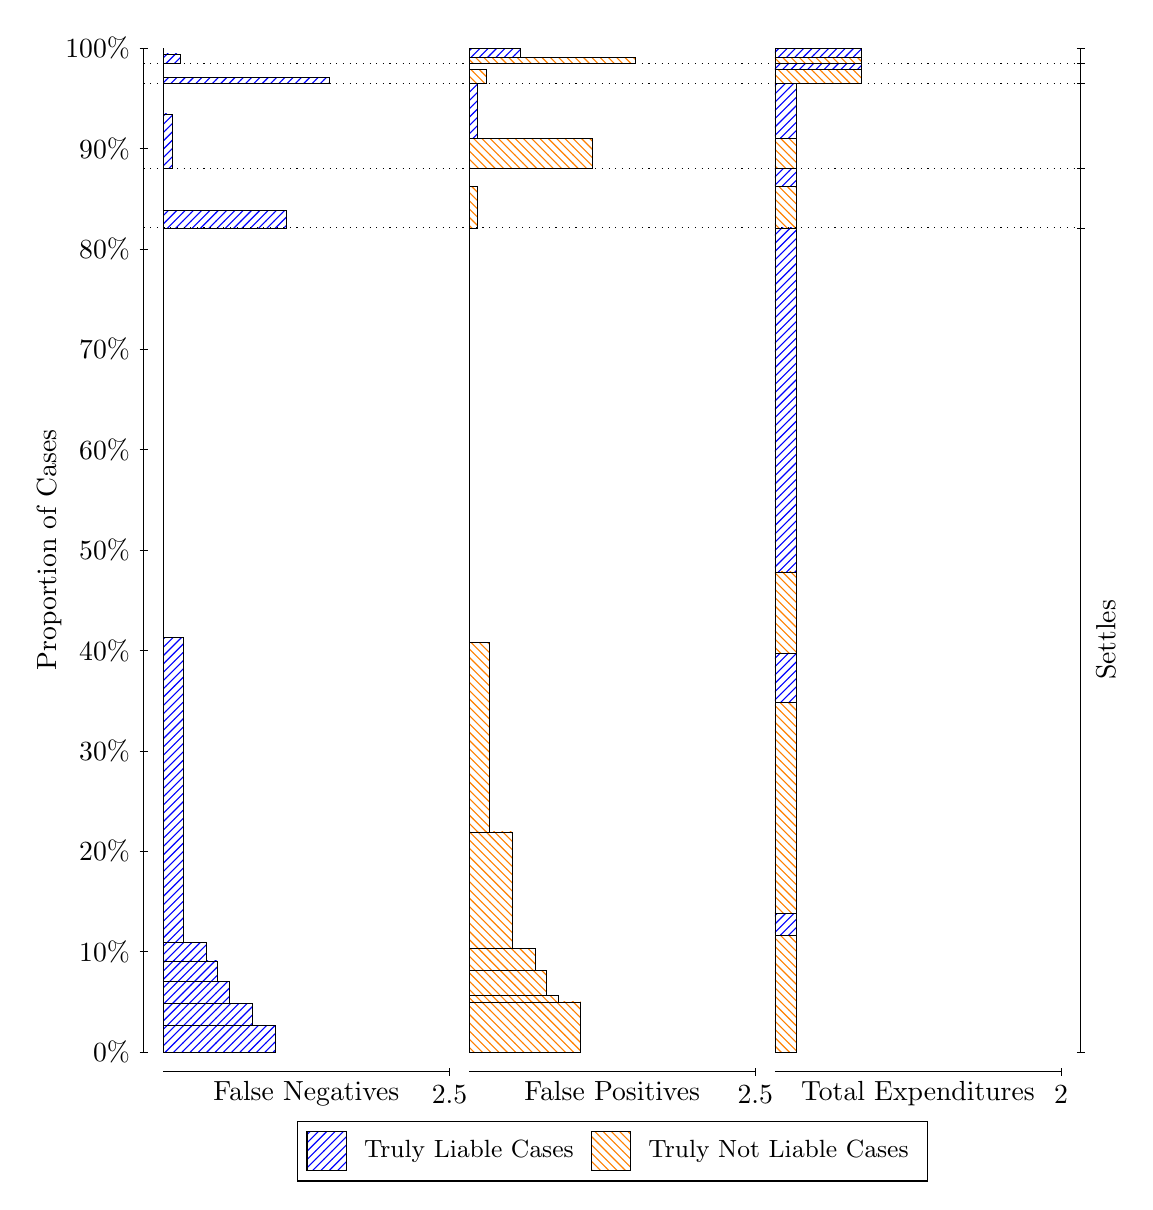
\begin{tikzpicture}
\draw[black, very thin] (1.5,1.75) -- (1.5,14.5);
\node[rotate=90, text=black, anchor=center] at (0.3, 8.125) {Proportion of Cases};
\draw[black, very thin] (1.45,1.75) -- (1.55,1.75);
\node[text=black, anchor=east] at (1.45, 1.75) {0\%};
\draw[black, very thin] (1.45,3.025) -- (1.55,3.025);
\node[text=black, anchor=east] at (1.45, 3.025) {10\%};
\draw[black, very thin] (1.45,4.3) -- (1.55,4.3);
\node[text=black, anchor=east] at (1.45, 4.3) {20\%};
\draw[black, very thin] (1.45,5.575) -- (1.55,5.575);
\node[text=black, anchor=east] at (1.45, 5.575) {30\%};
\draw[black, very thin] (1.45,6.85) -- (1.55,6.85);
\node[text=black, anchor=east] at (1.45, 6.85) {40\%};
\draw[black, very thin] (1.45,8.125) -- (1.55,8.125);
\node[text=black, anchor=east] at (1.45, 8.125) {50\%};
\draw[black, very thin] (1.45,9.4) -- (1.55,9.4);
\node[text=black, anchor=east] at (1.45, 9.4) {60\%};
\draw[black, very thin] (1.45,10.675) -- (1.55,10.675);
\node[text=black, anchor=east] at (1.45, 10.675) {70\%};
\draw[black, very thin] (1.45,11.95) -- (1.55,11.95);
\node[text=black, anchor=east] at (1.45, 11.95) {80\%};
\draw[black, very thin] (1.45,13.225) -- (1.55,13.225);
\node[text=black, anchor=east] at (1.45, 13.225) {90\%};
\draw[black, very thin] (1.45,14.5) -- (1.55,14.5);
\node[text=black, anchor=east] at (1.45, 14.5) {100\%};

\draw[black, very thin] (13.4,1.75) -- (13.4,14.5);
\draw[black, very thin] (13.35,1.75) -- (13.45,1.75);
\node[anchor=west] at (13.35, 1.75) {};
\draw[black, very thin] (13.35,12.217) -- (13.45,12.217);
\node[anchor=west] at (13.35, 12.217) {};
\draw[black, very thin] (13.35,12.967) -- (13.45,12.967);
\node[anchor=west] at (13.35, 12.967) {};
\draw[black, very thin] (13.35,14.05) -- (13.45,14.05);
\node[anchor=west] at (13.35, 14.05) {};
\draw[black, very thin] (13.35,14.306) -- (13.45,14.306);
\node[anchor=west] at (13.35, 14.306) {};
\draw[black, very thin] (13.35,14.5) -- (13.45,14.5);
\node[anchor=west] at (13.35, 14.5) {};

\draw[black, very thin, pattern color=blue, pattern=north east lines] (1.75,1.75) rectangle (3.167,2.0913);
\draw[black, very thin, pattern color=blue, pattern=north east lines] (1.75,2.0913) rectangle (2.8763,2.367);
\draw[black, very thin, pattern color=blue, pattern=north east lines] (1.75,2.367) rectangle (2.5857,2.6416);
\draw[black, very thin, pattern color=blue, pattern=north east lines] (1.75,2.6416) rectangle (2.4403,2.9075);
\draw[black, very thin, pattern color=blue, pattern=north east lines] (1.75,2.9075) rectangle (2.295,3.1418);
\draw[black, very thin, pattern color=blue, pattern=north east lines] (1.75,3.1418) rectangle (2.0043,7.0109);
\draw[black, very thin, pattern color=orange, pattern=north west lines] (1.75,7.0109) rectangle (1.75,12.217);
\draw[black, very thin, pattern color=blue, pattern=north east lines] (1.75,12.217) rectangle (3.3123,12.439);
\draw[black, very thin, pattern color=orange, pattern=north west lines] (1.75,12.439) rectangle (1.75,12.967);
\draw[black, very thin, pattern color=blue, pattern=north east lines] (1.75,12.967) rectangle (1.859,13.664);
\draw[black, very thin, pattern color=orange, pattern=north west lines] (1.75,13.664) rectangle (1.75,14.05);
\draw[black, very thin, pattern color=blue, pattern=north east lines] (1.75,14.05) rectangle (3.8573,14.124);
\draw[black, very thin, pattern color=orange, pattern=north west lines] (1.75,14.124) rectangle (1.75,14.306);
\draw[black, very thin, pattern color=blue, pattern=north east lines] (1.75,14.306) rectangle (1.968,14.426);
\draw[black, very thin, pattern color=orange, pattern=north west lines] (1.75,14.426) rectangle (1.75,14.5);
\draw[black, very thin, pattern color=orange, pattern=north west lines] (5.6333,1.75) rectangle (7.0503,2.3852);
\draw[black, very thin, pattern color=orange, pattern=north west lines] (5.6333,2.3852) rectangle (6.7597,2.4674);
\draw[black, very thin, pattern color=orange, pattern=north west lines] (5.6333,2.4674) rectangle (6.6143,2.788);
\draw[black, very thin, pattern color=orange, pattern=north west lines] (5.6333,2.788) rectangle (6.469,3.0626);
\draw[black, very thin, pattern color=orange, pattern=north west lines] (5.6333,3.0626) rectangle (6.1783,4.5462);
\draw[black, very thin, pattern color=orange, pattern=north west lines] (5.6333,4.5462) rectangle (5.8877,6.9563);
\draw[black, very thin, pattern color=blue, pattern=north east lines] (5.6333,6.9563) rectangle (5.6333,12.217);
\draw[black, very thin, pattern color=orange, pattern=north west lines] (5.6333,12.217) rectangle (5.7423,12.744);
\draw[black, very thin, pattern color=blue, pattern=north east lines] (5.6333,12.744) rectangle (5.6333,12.967);
\draw[black, very thin, pattern color=orange, pattern=north west lines] (5.6333,12.967) rectangle (7.1957,13.352);
\draw[black, very thin, pattern color=blue, pattern=north east lines] (5.6333,13.352) rectangle (5.7423,14.05);
\draw[black, very thin, pattern color=orange, pattern=north west lines] (5.6333,14.05) rectangle (5.8513,14.232);
\draw[black, very thin, pattern color=blue, pattern=north east lines] (5.6333,14.232) rectangle (5.6333,14.306);
\draw[black, very thin, pattern color=orange, pattern=north west lines] (5.6333,14.306) rectangle (7.7407,14.38);
\draw[black, very thin, pattern color=blue, pattern=north east lines] (5.6333,14.38) rectangle (6.2873,14.5);
\draw[black, very thin, pattern color=orange, pattern=north west lines] (9.5167,1.75) rectangle (9.7892,3.2336);
\draw[black, very thin, pattern color=blue, pattern=north east lines] (9.5167,3.2336) rectangle (9.7892,3.5092);
\draw[black, very thin, pattern color=orange, pattern=north west lines] (9.5167,3.5092) rectangle (9.7892,6.1939);
\draw[black, very thin, pattern color=blue, pattern=north east lines] (9.5167,6.1939) rectangle (9.7892,6.8099);
\draw[black, very thin, pattern color=orange, pattern=north west lines] (9.5167,6.8099) rectangle (9.7892,7.8479);
\draw[black, very thin, pattern color=blue, pattern=north east lines] (9.5167,7.8479) rectangle (9.7892,12.217);
\draw[black, very thin, pattern color=orange, pattern=north west lines] (9.5167,12.217) rectangle (9.7892,12.744);
\draw[black, very thin, pattern color=blue, pattern=north east lines] (9.5167,12.744) rectangle (9.7892,12.967);
\draw[black, very thin, pattern color=orange, pattern=north west lines] (9.5167,12.967) rectangle (9.7892,13.352);
\draw[black, very thin, pattern color=blue, pattern=north east lines] (9.5167,13.352) rectangle (9.7892,14.05);
\draw[black, very thin, pattern color=orange, pattern=north west lines] (9.5167,14.05) rectangle (10.607,14.232);
\draw[black, very thin, pattern color=blue, pattern=north east lines] (9.5167,14.232) rectangle (10.607,14.306);
\draw[black, very thin, pattern color=orange, pattern=north west lines] (9.5167,14.306) rectangle (10.607,14.38);
\draw[black, very thin, pattern color=blue, pattern=north east lines] (9.5167,14.38) rectangle (10.607,14.5);
\draw[black, dotted] (1.5,12.217) -- (13.4,12.217);
\draw[black, dotted] (1.5,12.967) -- (13.4,12.967);
\draw[black, dotted] (1.5,14.05) -- (13.4,14.05);
\draw[black, dotted] (1.5,14.306) -- (13.4,14.306);
\draw[black, very thin] (1.75,1.5) -- (5.3833,1.5);
\node[text=black, anchor=north] at (3.5667, 1.5) {False Negatives};
\draw[black, very thin] (5.3833,1.45) -- (5.3833,1.55);
\node[text=black, anchor=north] at (5.3833, 1.45) {2.5};

\draw[black, very thin] (5.6333,1.5) -- (9.2667,1.5);
\node[text=black, anchor=north] at (7.45, 1.5) {False Positives};
\draw[black, very thin] (9.2667,1.45) -- (9.2667,1.55);
\node[text=black, anchor=north] at (9.2667, 1.45) {2.5};

\draw[black, very thin] (9.5167,1.5) -- (13.15,1.5);
\node[text=black, anchor=north] at (11.333, 1.5) {Total Expenditures};
\draw[black, very thin] (13.15,1.45) -- (13.15,1.55);
\node[text=black, anchor=north] at (13.15, 1.45) {2};

\node[text=black, centered, rotate=90] at (13.72, 6.9836) {Settles};





\draw (7.449999999999999,1.5) node[draw=none] (baseCoordinate) {};
\begin{scope}[align=center]
        \matrix[scale=0.5, draw=black, below=0.5cm of baseCoordinate, nodes={draw}, column sep=0.1cm]{
            \node[rectangle, draw, minimum width=0.5cm, minimum height=0.5cm, pattern color=blue, pattern=north east lines] {}; &
            \node[draw=none, font=\small, text=black] (B) {Truly Liable Cases}; &
            \node[rectangle, draw, minimum width=0.5cm, minimum height=0.5cm, pattern color=orange, pattern=north west lines] {}; &
            \node[draw=none, font=\small, text=black] (B) {Truly Not Liable Cases}; \\
            };
\end{scope}

\end{tikzpicture}
\end{document}